\documentclass[]{article}
\usepackage{geometry}
\usepackage{amsmath}
\usepackage{newtxtext,newtxmath}
%\usepackage{newpxtext,newpxmath}
\usepackage{natbib}
\usepackage[justification=justified]{caption}
\usepackage{booktabs}
\usepackage{placeins}
\usepackage{xcolor}
%\usepackage{pdflscape}
\usepackage{rotating}
\usepackage{xr}
\geometry{a4paper, top=25mm, bottom=25mm, left=25mm, right=25mm}
\setlength{\parindent}{0.1cm}

%opening
\title{Approximations of the CME}
\author{}

\begin{document}

\maketitle

\section{Description of the Birth-Death chemical master equation}
The system consists of a molecular species with a count variable \(n\). There are two reactions:
\begin{enumerate}
	\item \textbf{Birth reaction:} Increases the molecule count by 1. Rate: \(\lambda_b(n) = n \times \max[0, k+C_b(N_{ss}-n)]\)
	\item \textbf{Death reaction:} Decreases the molecule count by 1. Rate: \(\lambda_d(n) = n \times k\)
\end{enumerate}

\subsection{Gillespie Algorithm}
The Gillespie algorithm can be used to simulate the stochastic dynamics of the system. The steps are:

\begin{enumerate}
	\item Initialize the molecule count \(n(0)\) at time \(t=0\).
	
	\item At each time step, calculate the rates of the birth and death reactions:
	\begin{enumerate}
		\item \(\lambda_b(n) = n \times \max[0, k+C_b(N_{ss}-n)]\)
		\item \(\lambda_d(n) = n \times k\)
	\end{enumerate}
	
	
	\item Construct a discrete distribution for the two reactions, with probabilities:
	
	\begin{enumerate}
		\item $ P[birth] = \lambda_b(n)/[\lambda_b(n) + \lambda_d(n)] $
		\item $ P[death] = \lambda_d(n)/[\lambda_b(n) + \lambda_d(n)] $
	\end{enumerate}
	
	And determine which reaction occurs by randomly drawing a sample. Update $n$ accordingly. 
	
	\item Calculate the time until the next reaction by randomly drawing a sample from an exponential distribution with rate $\lambda = \lambda_b(n) + \lambda_d(n)$, and update time accordingly. 
	
	\item Return to step 2 until desired simulation time is reached.
\end{enumerate}

\section{Deriving the Langevin approximation to the CME}

Consider a birth-death model where the birth rate \( k_b \) and death rate \( k_d \) are functions of \( n \), i.e., \( k_b(n) \) and \( k_d(n) \). We can express the general model as an approximated Langevin equation:

\begin{equation}
	dn = f(n) dt + g(n) \xi \sqrt{dt}
\end{equation}

Where:
\begin{itemize}
	\item \( f(n) \) is the deterministic drift term representing the net change rate of \( n \) due to both birth and death reactions.
	\item \( g(n) \) represents the strength of the noise term.
	\item \(\xi \sqrt{dt}\) is a standard normal random variable driving the randomness of the system.
\end{itemize}

\subsection{The drift term}

\subsubsection{Deriving $f(n)$}

The deterministic drift term $f(n)$ is the expected change in $n$ at each potential value of $n$. As such, it can be expressed as the negative difference between the expected number of birth and death events at that point. 

\begin{equation} \label{eq:term_drift} 
	f(n) = k_b(n) - k_d(n) = max[0, k + C_b \times (NSS-n)] \times n - k \times n
\end{equation}

\subsubsection{Exploring $f(n)$}

The shape and magnitude of the drift term function $f(n)$ is highly dependant on two parameters of the equation system, namely the control strength $C_b$, and the basal rates of births and deaths $k$ $( = k = k$)(Fig. \ref{fig:drift_depend}).

\begin{figure} [h] 
	\centering %
	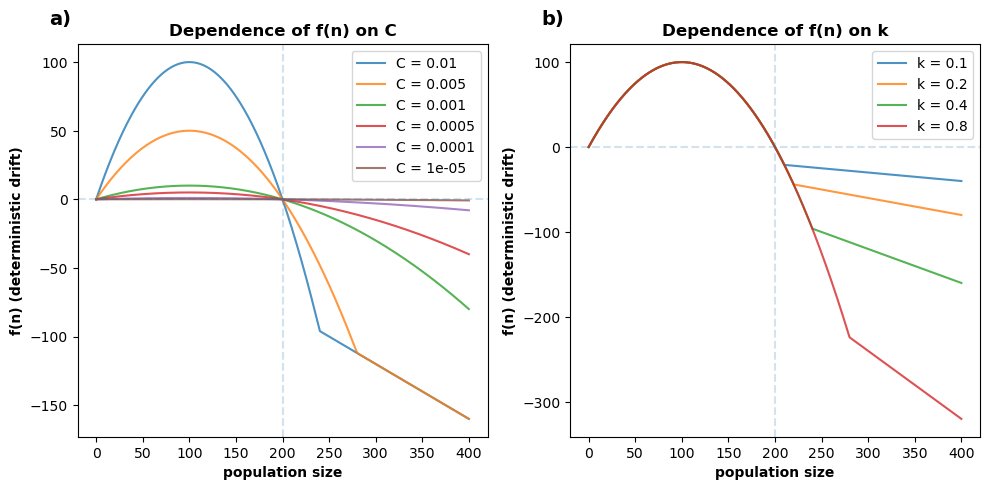
\includegraphics[scale=0.65]{figs/drift_dependence} 
	\caption{
		Dependence of drift term $f(n)$ on the control strength $C$ and turnover $k$.
		\textbf{a)} $f(n)$ across various values of $C_b$ when $k = 0.4$
		\textbf{b)} $f(n)$ across various values of $k$ when $C_b = 0.01$
	} 
	\label{fig:drift_depend}
\end{figure}

\subsection{The noise term $g(n)$}

The \( g(n) \) term in the Langevin equation captures the variance of the noise, i.e., the inherent stochasticity in the birth-death model. 

\subsubsection{deriving $g(n)$}

Given that the fluctuations in \( n \) arise due to stochastic birth and death events, we can derive \( g(n) \) by considering the variance in the changes of \( n \) during a small time interval \( dt \).

\subsubsection*{Expectation and Variance of \( \Delta n \)}

For a birth event, \( \Delta n = +1 \) occurs at rate \( k(n) \) and for a death event, \( \Delta n = -1 \) occurs at rate \( k(n) \). Therefore $E[\Delta n]$ is:

\begin{equation}
	E[\Delta n] = (+1) \cdot k(n) \cdot dt + (-1) \cdot k(n) \cdot dt = (k(n) - k(n)) \cdot dt
\end{equation}

Accordingly, the second moment is:
\begin{equation}
	E[(\Delta n)^2] = (1^2) \cdot k(n) \cdot dt + (-1^2) \cdot k(n) \cdot dt = (k(n) + k(n)) \cdot dt
\end{equation}

And the variance \( \text{Var}[\Delta n] \) in \( n \) during \( dt \) is:

\begin{equation}
	\text{Var}[\Delta n] = E[(\Delta n)^2] - [E[\Delta n]]^2 = (k(n) + k(n)) \cdot dt - [(k(n) - k(n)) \cdot dt]^2
\end{equation}

Substituting $k(n) = n \cdot max[0, k + C_b \cdot (NSS-n)]$ and $k(n) = n \cdot k$ yields:

\begin{equation}
	\text{Var}[\Delta n] = (n \cdot max[0, k + C_b \cdot (NSS-n)] + n \cdot k) \cdot dt - [n \cdot max[0, k + C_b \cdot (NSS-n)] - n \cdot k) \cdot dt]^2
\end{equation}

Which can be expanded and rearranged to give:

\begin{equation}
\begin{aligned}
\text{Var}[\Delta n] = &  n \cdot (\max [0,k+C_b (NSS-n)] dt + k) dt + \\
	 & n^2 \cdot (2 k \max [0,k+C_b (NSS-n)] - k^2 - \max [0,k+C_b (NSS-n)]^2) dt^2  
\end{aligned}
\end{equation}

A suitable linear approximation of \( \text{Var}[\Delta n] \) is therefore:

\begin{equation} \label{eq:delta_n_variance}
	\text{Var}[\Delta n] \approxeq  n \cdot (\max [0,k+C_b (NSS-n)] dt + k) dt
\end{equation}

\subsubsection*{Deriving \( g(n) \) from \( Var[\Delta n]\)}

In the Langevin equation, the term \( g(n) \xi \sqrt{dt} \) represents the stochastic or random change in \( n \) over that same time increment. Thus the variance of $\Delta n$ can be expressed as:

\begin{equation}
	\Delta n = g(n) \xi \sqrt{dt} \implies Var[\Delta n] = Var[g(n) \xi \sqrt{dt}]
\end{equation}

Since \( \xi \) is a standard normal random variable with variance 1:

\begin{equation}
	\text{Var}[\Delta n] = \text{Var}[g(n) \xi \sqrt{dt}] = g(n)^2 \text{Var}[\xi] dt = g(n)^2 dt
\end{equation}

Substituting back eq. \ref{eq:delta_n_variance} and diving by $dt$:

\begin{equation}
	g(n)^2 = \text{Var}[\Delta n]/dt = \frac{n \cdot (\max [0,k+C_b (NSS-n)] dt + k) dt}{dt} = n \cdot (\max [0,k+C_b (NSS-n)] dt + k)
\end{equation}

Taking the square root finally gives:

\begin{equation} \label{eq:g_n_squared}
	g(n) =  \sqrt{n \cdot (\max [0,k+C_b (NSS-n)] dt + k)}
\end{equation}

\subsubsection{Exploring $g(n)$}

The shape and magnitude of the noise term $g(n)$ is dependant on two parameters of the equation system, namely the control strength $C_b$, and the basal rates of births and deaths $k$ $( = k = k$)(Fig. \ref{fig:noise_depend}).

\begin{figure} [h] 
	\centering %
	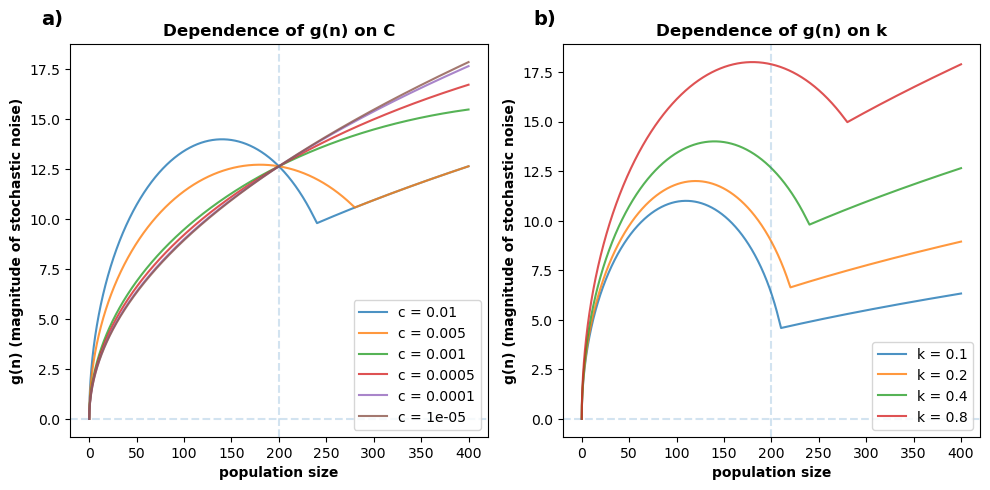
\includegraphics[scale=0.65]{figs/noise_dependence} 
	\caption{
		Dependence of the noise term $g(n)$ on the control strength $C$ and turnover $k$. 
		\textbf{a)} $g(n)$ across various values of $C_b$ when $k = 0.4$
		\textbf{b)} $g(n)$ across various values of $k$ when $C_b = 0.01$
	}. 
	\label{fig:noise_depend}
\end{figure}

\subsection{Complete equation}

Combinding the deterministic drift term, and the stochastic change yields the complete SDE describing the change in population size over time:

\begin{equation} \label{eq:langevin_full}
	dn = n \cdot (max[0, k + C_b \cdot (NSS-n)] - k) dt + \sqrt{n \cdot (\max [0,k+C_b (NSS-n)] dt + k)} \cdot  \xi \sqrt{dt}
\end{equation}

\subsection{Simulation using the Euler-Maruyama method}

We wish to approximate the SDE defined by eq. \ref{eq:langevin_full}. Using the  Euler-Maruyama method.

\begin{equation}
	\Delta n = f(n) \Delta t + g(n) \xi \sqrt{\Delta t}
\end{equation}

\subsubsection{Update equation}



When the system is simulated using the Euler-Maruyama method, the drift term becomes:

\begin{equation} \label{eq:term_drift} 
	f(n)\Delta t = n \cdot (max[0, k + C_b \cdot (NSS-n)] - k) \Delta t
\end{equation}

The magnitude of the noise term is calculated as:

\begin{equation} \label{eq:magnitude_noise} 
	g(n) = \sqrt{n\cdot(max[0, k + C_b \cdot (NSS-n)] + k)}
\end{equation}

Which is then multiplied by a sample taken from a standard normal distribution, and the square root of the timestep to yield the noise term:

\begin{equation} \label{eq:term_noise} 
	g(n) \xi \sqrt{\Delta t} = \sqrt{n\cdot(max[0, k + C_b \cdot (NSS-n)] + k)} \cdot  \xi \sqrt{\Delta t}
\end{equation}

Therefore the complete update equation for a discrete time step is:

\begin{equation} \label{eq:EM_update} 
	n_{t + \Delta t} = n_t + n (max[0, k + C_b \cdot (NSS-n)] - k)\Delta t + \sqrt{n(max[0, k + C_b \cdot (NSS-n)] + k)} \cdot \xi \sqrt{\Delta t} 	
\end{equation}


\section{ Continuous-Time Markov Chain representation of the CME}

In stochastic modelling, a birth-death process can be approximated by a Continuous-Time Markov Chain (CTMC), due to the memoryless property, the natural incorporation of time-dependent transition rates, and the discretized state space of the original birth-death process. 

In a birth-death process, entities can "birth" into or "die" out of various states at specific rates. These rates can be encapsulated in a transition rate matrix \( Q \), which provides a compact and mathematically tractable way to describe the system's dynamics. The CTMC framework allows for the analytical solution of various performance metrics, such as state probabilities through the use of differential equations and matrix exponentials.

Moreover, CTMCs offer a high degree of flexibility in modeling different kinds of birth-death processes, including those with state-dependent rates, multiple types of transitions, and more complex state spaces. Therefore, the CTMC serves as a robust and versatile framework for approximating birth-death processes, providing both conceptual clarity and analytical solutions.

\subsection{Defining the state space $S$}

Due to the way in which birth rates are specified, there are two boundaries in the state space of the birth-death process. The first trivial boundary is the absorbing state $n_{min} = 0$. The second boundary occurs when the birth rate drops to 0, above which the population size cannot grow.

\begin{equation}
	k_b(n) = 0 \implies n \cdot max[0, k + C_b \cdot (NSS-n)] = 0 \implies n_{max} = NSS + \frac{k}{C_b}
\end{equation}

Therefore, the corresponding set of all states for the CTMC is $S = \{0, 1, 2, ..., n_{max} \}$, and the transition rate matrix $Q$ will have size $n_{max} + 1$

\subsection{Defining the transition rate matrix $Q$}

As Each state $i$ of the CTMC corresponds to a given population size $n$ in the birth-death process, transitions between different states of the Markov Chain $q_{i,j}$ correspond to singular birth and death events which change the population size by 1. As discussed previously, these the rate of these events ($\lambda_b, \lambda_d$) themselves are dependant on the population size at which the events occur ($\lambda_b(n), \lambda_d(n)$). Therefore, the transition rate matrix $Q$ is defined as:

\begin{equation}
	Q = \left( q_{ij} \right)_{0 \leq i, j \leq N} \text{ where }
	\begin{cases}
		q_{0,j} = 0, & \text{for all $j$, since $i = 0$ is absorbing} \\
		q_{i, j = i+1} = \lambda_b(i) = i \cdot max[0, k + C_b \cdot (NSS-i)], & \text{for $i > 0$, the rate of birth events} \\
		q_{i, j = i-1} = \lambda_d(i) = i \cdot k, & \text{for $i > 0$, the rate of death events} \\
		q_{i, j} = 0, & \text{otherwise} \\
	\end{cases}
\end{equation}

To satisfy the properties of transition rate matrices, the additional constraint $q_{ii} = -\sum_{j \neq i} q_{ij}$ is also applied to give the tridiagonal matrix:

\begin{equation}
	Q = 
	\begin{pmatrix}
		0 & 0 & 0 & 0 & \cdots & 0 \\
		\lambda_d(1) & -q_1 & \lambda_b(1) & 0 & \cdots & 0 \\
		0 & \lambda_d(2) & -q_2 & \lambda_b(2) & \cdots & 0 \\
		0 & 0 & \lambda_d(3) & -q_3 & \cdots & 0 \\
		\vdots & \vdots & \vdots & \vdots & \ddots & \vdots \\
		0 & 0 & 0 & 0 & \lambda_d(n_{max}) & -\lambda_d(n_{max})
	\end{pmatrix}
\end{equation}

\subsection{Defining the transition probability matrix over time $P(t)$}

A fundamental result in the theory of CTMCs arises from the solution to the continuous-time Chapman-Kolmogorov equation. Given the infinitesimal generator matrix $Q$, the transition probability matrix at time $t$ can be obtained via a matrix exponential:

\begin{equation}	
	P(t) = e^{Q \cdot t}
\end{equation}
 
\subsection{Calculating the distribution of states over time $\pi(t)$}

The discrete distribution $\pi(t)$ corresponds to the state space S of the CTMC. Each element $\pi_i(t)$ represents the probability of the system being in state $i$ at time $t$. $\pi(t)$ is determined by the initial state distribution $\pi(0)$ and the transition probability matrix $P(t)$ according to:

\begin{equation}
	\pi(t) = \pi(0) \times P(t) \implies \pi(t) =  \pi(0) \times e^{Q \cdot t}
\end{equation}



\section{Results}

Simulations comparing the Gillespie system and the Langevin model show extremely close correspondence. At higher values of C, the approximation successfully recreates the slight but stable drop in population size (Fig. \ref{fig:match_1}), while at lower C values, the approximation successfully follows the exact decreasing trajectory (Fig. \ref{fig:match_2}). As $C$ nears 0, the approximation again recreates the lack of change in $n$ over time (Fig. \ref{fig:match_3}). 

\begin{figure} [h] 
	\centering %
	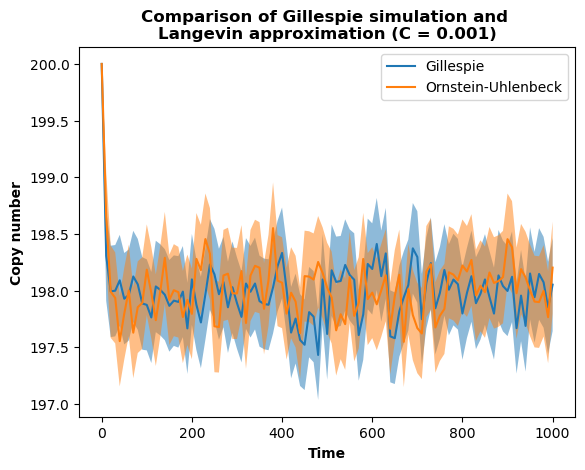
\includegraphics[scale=0.6]{figs/langevin_match_1} %
	\caption{Comparison of copy numbers over time at a high $C$ value. (10000 replicates, $k = 0.4$)} 
	\label{fig:match_1}
\end{figure}

\begin{figure} [h] 
	\centering %
	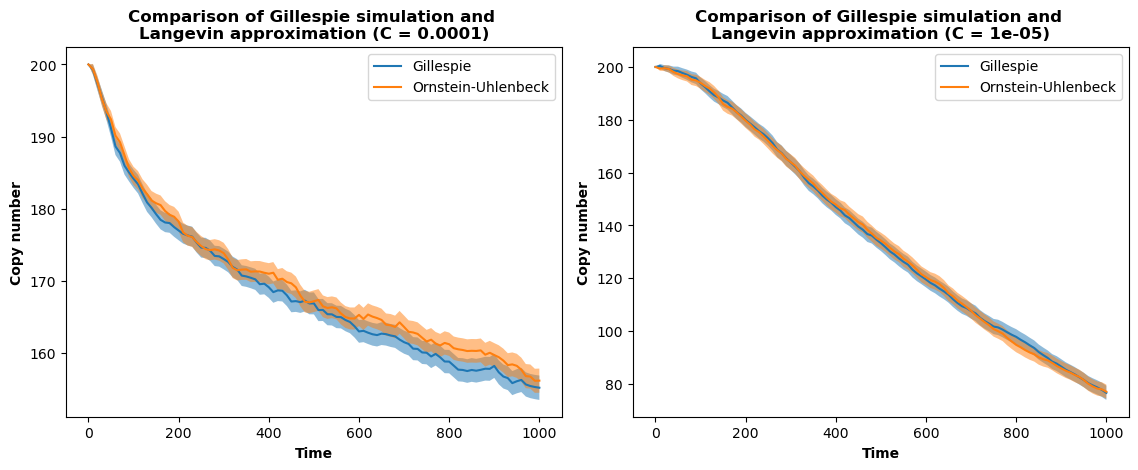
\includegraphics[scale=0.6]{figs/langevin_match_2} 
	\caption{Copy numbers decrease over time at lower $C$ values (10000 replicates, $k = 0.4$)} 
	\label{fig:match_2}
\end{figure}

\begin{figure} [h] 
	\centering %
	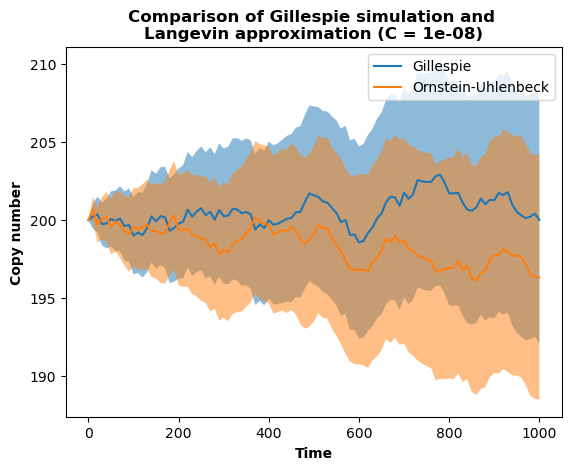
\includegraphics[scale=0.6]{figs/langevin_match_3} 
	\caption{Copy numbers are stagnant over time when $C \approxeq 0$ (10000 replicates, $k = 0.4$)} 
	\label{fig:match_3}
\end{figure}

\section{Interpretation}

These results suggest that the peculiar non-monotonic behaviour of $f(n, t)$ with respect to changes in $C_b$ observed in the Gillespie SSA are the result of the interaction between the restoring force $f(n)$, and the amount of stochastic variation $g(n)$.

\end{document}




















\newpage
\section{Ornstein-Uhlenbeck approximation}

\subsection{Introduction}

The changes in copy number of the system over time can be approximated as an Ornstein-Uhlenbeck process occurring in a given potential energy landscape. The change in copy number ($C$) is given by:

\begin{equation} \label{eq:o_u} 
	dC(t) = -\alpha \nabla U(C(t))dt + \sqrt{2 D} dW(t)
\end{equation} 

The gradient of the potential energy is defined for a given $C$ according to the expected change in $C$ due to the combined effects of actively controlled births, and deaths occurring with a constant rate:

\begin{equation} \label{eq:gradient} 
	\nabla U(C(t))dt = - C(max[0, Birth + C_b (NSS-C)] - Death)dt
\end{equation} 

Thus the full equation takes the form:

\begin{equation} \label{eq:o_u_full} 
	dC(t) = \alpha \times C(max[0, Birth + C_b (NSS-C)] - Death)dt + \sqrt{2 D} dW(t)
\end{equation} 

\newpage
\subsection{Parameter inference}

As the $Birth$, $Death$, $NSS$, and $C_b$ parameters are predetermined, simulating with the model requires the inference of the $D$ and $\alpha$ parameters. 

\subsubsection{Estimating D}
The estimation of $D$ is relatively straightforward. If $C_b = 0$, the probability of birth and death events is equal at all times, and $C$ simply reverts to 1-D Brownian motion. Therefore, $Var(C(t))$ is given by:

\begin{equation} \label{eq:D} 
	Var(C(t)) = 2Dt
\end{equation} 

The Gillespie algorithm can be used to simulate a high number ($10^5$) of replicates, which can then be used to infer $Var(C(t))$.  A visualization of the observed variance over time suggests that the Brownian motion assumptions are well founded. Therefore $D$ can be estimated as the best linear fit (with intercept 0) to the observed variance over time (eq. \ref{eq:D_fit}). This yields an estimate of $D \approx 85$.



\begin{figure}[h]
	\begin{center}
		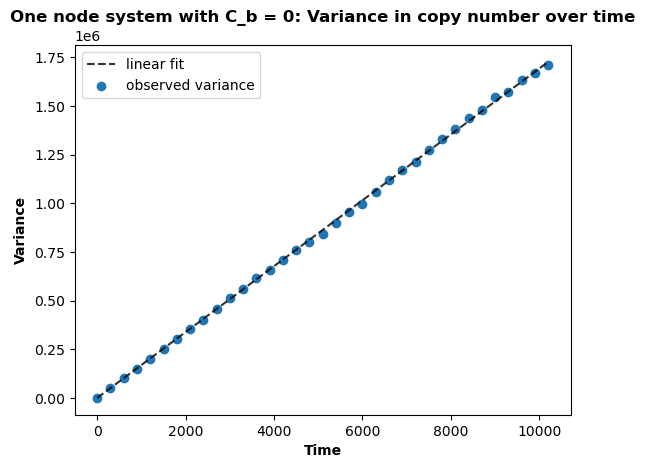
\includegraphics[scale=0.65]{figs/1node_variance} %
	\end{center}
	\caption{When $C_b = 0$, the variance of copy number over time is near linear.}
	\label{fig:variance}
\end{figure}


\begin{equation} \label{eq:D_fit} 
	2D = \frac{\sum_{i} t_i \times \hat{Var(C(t))_i}}{\sum_{i} t_i^2}
\end{equation} 

A series of simulations with varying $NSS$ and $Birth$ and $Death$ rates reveals:

\begin{equation} \label{eq:D_fit} 
	D \propto Turnover \times NSS
\end{equation} 

\subsubsection{Estimating $\alpha$}
???



\section*{Derivation of \(D\) for the Birth-Death Model}

\subsection*{1. Reaction Rates:}
The propensity for a birth event (increase of one molecule) is \(k \cdot n\). Similarly, the propensity for a death event (decrease of one molecule) is \(k \cdot n\).

Given the nature of the Gillespie algorithm, the time to the next reaction (either birth or death) is exponentially distributed with parameter \(2kn\). Thus, the mean time \( \tau \) to the next reaction is:
\begin{equation}
	\tau = \frac{1}{2kn}
\end{equation}

\subsection*{2. Change in the Number of Molecules (Random Walk Mapping):}
Every reaction changes \(n\) by \( \pm 1\). Given that both birth and death reactions are equally likely, the expected change \(E[\Delta n]\) in one step is 0. However, the variance of this change, \( \text{Var}(\Delta n) \), in one step is:
\begin{equation}
	\text{Var}(\Delta n) = E[(\Delta n)^2] - E[\Delta n]^2 = 1
\end{equation}

\subsection*{3. Relate to Diffusion in Continuous Time:}
Over a continuous time \(t\), there would be, on average, \( \frac{t}{\tau} \) reactions. Therefore, the variance in \(n\) over this time would be:
\begin{equation}
	\text{Var}(n(t)) = \frac{t}{\tau} \times \text{Var}(\Delta n) = 2kn \times t
\end{equation}

\subsection*{4. Relation to the Diffusion Constant:}
The variance in the number of molecules \(n(t)\) for a diffusive process is related to the diffusion constant \(D\) as:
\begin{equation}
	\text{Var}(n(t)) = 2Dt
\end{equation}
Equating the two expressions:
\begin{equation}
	2Dt = 2kn \times t
\end{equation}
From which we get:
\begin{equation}
	D = kn
\end{equation}

\subsection*{Conclusion:}
Given the rates \(k\) and the number of molecules \(n\) for the described birth-death process, the diffusivity constant \(D\) is simply the product of \(k\) and \(n\):
\begin{equation}
	D = kn
\end{equation}







\subsection{Deriving the variance of the noise term}

Due to the dynamic time step 

To derive \( g(n) \), the term capturing the variance of the inherent noise, we start by considering the changes in \( n \) due to stochastic birth and death events.


\subsubsection{Births:}
Consider a discrete time step \(dt\). The change in the number of molecules due to a birth event within this time step, \( \Delta n_{\text{birth}} \), can either be \( +1 \) (if a birth occurs) or \( 0 \) (if no birth occurs). The expected change due to a birth event is therefore the probability of a birth event occurring in the interval:

\begin{equation} \label{eq:expected_birth}
	E[\Delta n_{\text{birth}}] = k(n)dt = n \times max[0, k + C_b \times (NSS-n)] dt
\end{equation}

The variance in \( \Delta n_{\text{birth}} \) is:

\begin{equation} \label{eq:variance_birth}
	\text{Var}(\Delta n_{\text{birth}}) = E[\Delta n_{\text{birth}}^2] - (E[\Delta n_{\text{birth}}])^2
\end{equation}

Given that \( \Delta n_{\text{birth}} \) can either be \( +1 \) or \( 0 \), we can compute the second moment as:

\begin{equation}
	E[\Delta n_{\text{birth}}^2] = (+1)^2 \times k(n)dt + 0^2 \times (1 - k(n)dt) = k(n)dt
\end{equation}

Substituting back into eq. \ref{eq:variance_birth}, we get:

\begin{equation}
	\text{Var}(\Delta n_{\text{birth}}) = k(n)dt - (k(n)dt)^2
\end{equation}

And the full form of \( \text{Var}(\Delta n_{\text{birth}}) \) is: 

\begin{equation}
	\text{Var}(\Delta n_{\text{birth}}) = n \times max[0, k + C_b \times (NSS-n)] dt - n^2 \times max[0, k + C_b \times (NSS-n)]^2 dt^2
\end{equation}

Therefore, a linear approximation to \( \text{Var}(\Delta n_{\text{birth}}) \) is:

\begin{equation}
	\text{Var}(\Delta n_{\text{birth}}) \approxeq n \times max[0, k + C_b \times (NSS-n)] dt
\end{equation}


\subsubsection{Deaths:}
The change in number of molecules due to a death event within time step \(dt\), \( \Delta n_{\text{death}} \), can either be \( -1 \) (if a death occurs) or \( 0 \) (if no death occurs). The expected change due to a death event is:
\begin{equation}
	E[\Delta n_{\text{death}}] = -k(n)dt = n \times k dt
\end{equation}

The variance in \( \Delta n_{\text{death}} \) is:

\begin{equation}
	\text{Var}(\Delta n_{\text{death}}) = E[\Delta n_{\text{death}}^2] - (E[\Delta n_{\text{death}}])^2
\end{equation}

Given that \( \Delta n_{\text{death}} \) can either be \( -1 \) or \( 0 \), we can compute the second moment as:

\begin{equation}
	E[\Delta n_{\text{death}}^2] = (-1)^2 \times k(n)dt + 0^2 \times (1 - k(n)dt) = k(n)dt
\end{equation}

Substituting in, we get:

\begin{equation}
	\text{Var}(\Delta n_{\text{death}}) = k(n)dt - (k(n)dt)^2 = n \times k dt - n^2 k^2 dt^2
\end{equation}

Which can be linearly approximated as:

\begin{equation}
	\text{Var}(\Delta n_{\text{death}}) \approxeq n \times k dt
\end{equation}

\subsubsection{Total Variance:}
To get the total variance \( \text{Var}(\Delta n) \), we assume that birth and death processes are independent, and their variances are therefore additive. Thus, the linear approximation of $g(n)$ is:

\begin{equation}
	\text{Var}(\Delta n) = \text{Var}(\Delta n_{\text{birth}}) + \text{Var}(\Delta n_{\text{death}}) \approxeq n\times(max[0, k + C_b \times (NSS-n)] + k)dt
\end{equation}

\subsubsection{Total Variance:}
To get the total variance \( \text{Var}[\Delta n] \), we first consider the 

onsider a birth-death model where the birth rate \( k \) and death rate \( k \) are functions of \( n \), i.e., \( k(n) \) and \( k(n) \). The Langevin equation describes the system as:

\begin{equation}
	dn(t) = f(n) \, dt + \sqrt{g(n)} \, dW(t)
\end{equation}

Where \( f(n) = k(n) - k(n) \) is the deterministic drift term. To derive \( g(n) \), the term capturing the variance of the inherent noise, we start by considering the changes in \( n \) due to stochastic birth and death events.
